\chapter{Implementation of the solution}\label{ch:implementation-of-the-solution}
In order to implement a solution from chapter~\ref{ch:proposed-solution-to-problem}, a edge cloud computing environment
must be simulated due to the impractically of setting up such a network and in order to train the agents proposed
in section~\ref{sec:proposed-agents}. This chapter splits the implementation into three sections: the environment
simulation (section~\ref{sec:simulating-edge-cloud-computing-services}), define server auction agents and resource
allocation agents (section~\ref{sec:implementing-auction-and-resource-allocation-agents}) and finally training the
agents (section~\ref{sec:training-agents}).

The implementation discussed below as written in Python and available to download from Github at
\burl{https://github.com/stringtheorys/Online-Flexible-Resource-Allocation}. The reason for the use of python is number
of modules available for reinforcement learning and the speed of development.

\section{Simulating edge cloud computing services}\label{sec:simulating-edge-cloud-computing-services}
While the aim of the environment is the simulate accurately edge cloud computing server, the implementation of the
environment must allow agents to train on interact and training on the environment. Therefore it has been implemented
using as an OpenAI gym~\citep{openaigym}, the de facto standard for implementing reinforcement learning
environment for researchers. However the standard specification must be modified due to the problem being multi-agent,
multi-step and as a centralised system.

An example for running the environment is in figure~\ref{listing:example_flexible_resource_env}. There are three
sections to the code; the first is the construct an environment using the constructor, where the environment settings
are passed that determines the number of servers and tasks and there attributes. These attributes are determined using
uniform random numbers between a maximum and minimum values that are synthesis individually for each variable. The
second is to create the environment using the reset function returning the current environment state. The environment
state contains a task to be auctioned if any task's auction time step is equal to the environment's current time step
as well as a dictionary of server to their current state. Using these states, each server generate's actions either
using the auction agent or resource allocation agent depending if if task needs auctioning. The third step is to
take a step in environment using the server actions that returns an updated server state, the rewards for the actions,
if the environment is finished and an extra information from the steps taken. The rewards are a dictionary of each of
the servers with either the winning price for the auctioned task or a list of tasks that have finished either because
they ran out of time or completed the task early.

\begin{lstlisting}[language=Python, frame=single, caption={An example for running the environment},captionpos=b]
# Load the environment with a setting
env = OnlineFlexibleResourceAllocationEnv('settings.env')

# Generate the environment state
server_state = env.reset()

for _ in range(1000):
    # Generate actions
    if server_state.auction_task:
        actions = {
            server: auction_agent.bid(state)
            for server, state in server_state
        }
    else:
        actions = {
            server: resource_allocation_agent.weights(state)
            for server, state in server_state
        }

    # Take environment step
    server_state, reward, done, info = env.step(actions)

    # If the environment is finished then reset it
    if done:
        server_state = env.reset()
\label{listing:example_flexible_resource_env}
\end{lstlisting}

\subsection{Server resource allocation}\label{subsec:server-resource-allocation}
A particular complication of the system is to distribute server resources due to the fact that server provide a
dictionary of task with a resource weighting that much be converted to the allocated resources for each task.
To allocate the compute resources is relatively simple compared to allocating resources for both storage and bandwidth.
The algorithm checks first if the weighted resources is greater than the quantity required for the task to finish the
compute stage, if this is true then a resources needed for the task to complete the compute stage are allocated. However,
this means that the weight resources available for each task is increased due to a task not using all of the resources
it could. This means that the algorithm loops till no task can be completed with the weighted resources allocated.
Then all of the reminding compute resources are allocated to the remaining tasks.

For allocating storage and bandwidth, the reason for this being more difficult is due to when the server is still
loading the task, the server must allocate both storage and bandwidth resources while the bandwidth must be allocated
to the task sending results. Because of this, a tension exists between these two operation for allocating resources.
The implemented algorithm, gives priority for allocating resources to the tasks sending results as these tasks are more
likely to be finished and will not penalise the server for not completing the task within the deadline. To allocate
resources, a similar function to used to the one for allocating compute resources. First a check if done using the
weighted bandwidth resources to see if any task sending results will be finished with the resources, if so these
resources are allocated. This process if repeat for the server loading any task with the additional check that there
is enough available storage for the bandwidth resources being allocated. For any remaining task, this process if
repeated till all of the available resources are allocated in the time step. As a results, using this algorithm, the
converting between weightings to resources allowing for allocating of almost all of the server's resources with no
resources unused.

\section{Implementing Auction and resource allocation agents}\label{sec:implementing-auction-and-resource-allocation-agents}
Each server has to have a unique policy for bidding on tasks and allocating resources that are proposed in
section~\ref{sec:proposed-agents}. These policies are referred to as the auction agents, for bidding on tasks and the
resource weighting agent, for allocating of resources. However determining these policies is a difficult due to the
complexity and the interaction of task attributes and the server resources. Because of this, the ability of
reinforcement learning to interact an environment and learn a policy in order to maximise its reward over time is
integral to this project. Therefore a range of different reinforcement learning techniques have been implemented,
outlined in Table~\ref{tab:reinforcement_learning_algorithms}, in order to explore the different options that a server
would have available to learn its policies.

% Todo auction and resource allocation agents

\subsection{Implementing reinforcement learning policies}\label{subsec:implementing-auction-and-resource-allocation-agents}
These policies were implemented using tensorflow~\cite{tensorflow2015-whitepaper}, a python module developed by Google
that provides programmers the ability to construct neural network and backpropagation with a loss function. A
particular problem with this project is the use of recurrent neural network and inputs not having a fixed length. This
causes an issue with tensorflow due to the requirement for tensor, the base for tensorflow operation, to have a fixed
size. To allow for efficient using of backpropagation with multiple inputs being computed at the same time in order to
compute a minibatch not just stochastic gradient descent. To do requires the use of the tensorflow preprocessing module
to pad all of the input to be the same size.

\begin{table}
    \centering
    \begin{tabular}{|p{3cm}|p{12cm}|} \hline
        Policy Type & Explanation \\ \hline
        Dqn~\citep{mnih2015humanlevel} & A standard deep Q learning agent that discretizes the action space \\ \hline
        Double Dueling DQN~\citep{doubledqn, duelingdqn} & A combination of two heuristics for the standard deep Q
            learning agents that uses a modified td target function and a modified networks that separates state value
            and action advantage. \\ \hline
        Categorical Dqn~\citep{distributional_dqn} & Standard deep Q learning agents return a scalar value
            (representing the q value) for each action. Distributional Dqn changes the output value to a probability
            distribution over action values that is helpful due to the stochastic nature from the problem (from the
            agents perspective). \\ \hline
        Deep deterministic policy gradient~\citep{ddpg} & As the action space is continuous, DDPG allows for
            investigation of the difference between continuous and discrete action spaces of the DQN agents and policy
            gradient can be more effective at learning a policy where the reward function is too complex for DQN to
            model. \\ \hline
        Twin delay DDPG~\citep{td3} & Like the Double Dueling DQN agents, TD3 includes a couple new heuristics, like a
            twin critic to prevent the actor tricking the critic and delaying the updates for actors compared to
            critic.\\ \hline
        D4PG~\citep{d4pg} & Like the categorical dqn, d4pg add a heuristic for the critic to output a value probability
            distribution that allows for better approximation for environment that are stochastic in nature. \\ \hline
    \end{tabular}
    \caption{Table of implemented reinforcement learning algorithms}
    \label{tab:reinforcement_learning_algorithms}
\end{table}

\subsection{Rewards functions}\label{subsec:rewards-functions}
As explained in the background review for reinforcement learning (section~\ref{sec:related-work-in-machine-learning}),
the q values is an approximation for the estimated discounted reward in the future given an action. Therefore the
rewards that an agent receives for taking an action is extremely important to enable the agent to learn. This problem
of complex reward functions are a known problem for DQN agent to deal with~\citep{atari} while policy gradients can
deal with this due to learning the policy rather than the q values~\citep{Sutton1998}.

For the auction, the reward is based on the winning price of the task at the time step when the auction is won. If the
task fails, the reward is instead multiplied by a negative constant (referred to as "failed\_reward\_multiplier") in
order to discourage the auction agent from bidding on tasks that it wouldn't be able to complete. Because of this,
the price of zero is treated as a non-bid, resulting in the agent getting a reward of zero and not being considered in
the auction. The final possible reward for an auction agent is that the agent fails to win the task in the auction by
bidding too high, as a result, the reward is constant called "failed\_auction\_reward". The constant's default value is
-0.05 as a way of encouraging the agent to change there bid.

For resource allocation, the reward function is much simpler than the auction reward function as it only needs to
consider the task being weighted at the time and rewards from other tasks allocated at the time. This is as,
a task must consider its actions in consider with the resource requirements of other allocated tasks. For successfully
finishing a task, the reward is 1 while the reward for if the task has failed is -1.5 to make failing a task more
costly than completing a task. But when a task's action is not under consideration, this reward is multiplied by
0.4 as while this rewards impact the task, their value is not as important to the task current consideration.
While these rewards don't consider the price payed for the task instead valuing each task equally with the aim of
forcing the task allocate resources to finish all tasks not just the valuable ones. Using this information, the reward
function simply just the sum of finished tasks rewards in the next time step.

\subsection{Agent observations}\label{subsec:agent-observations}
Both deep q networks and policy gradient algorithm are based on the Q function (explained in
section~\ref{sec:related-work-in-machine-learning})) which tries to approximate the reward at the next time step. To do
this required a reward function and a next observation to compare to in order to train these agents. This can be
described as a tree with the current state being the root and all lefts being the next states however for this problem,
this formulation has several problems due to there being two environment happening at the same time meaning that the
next state is not clear as shown in figure~\ref{fig:environment-observations}.

\begin{figure}
    \centering
    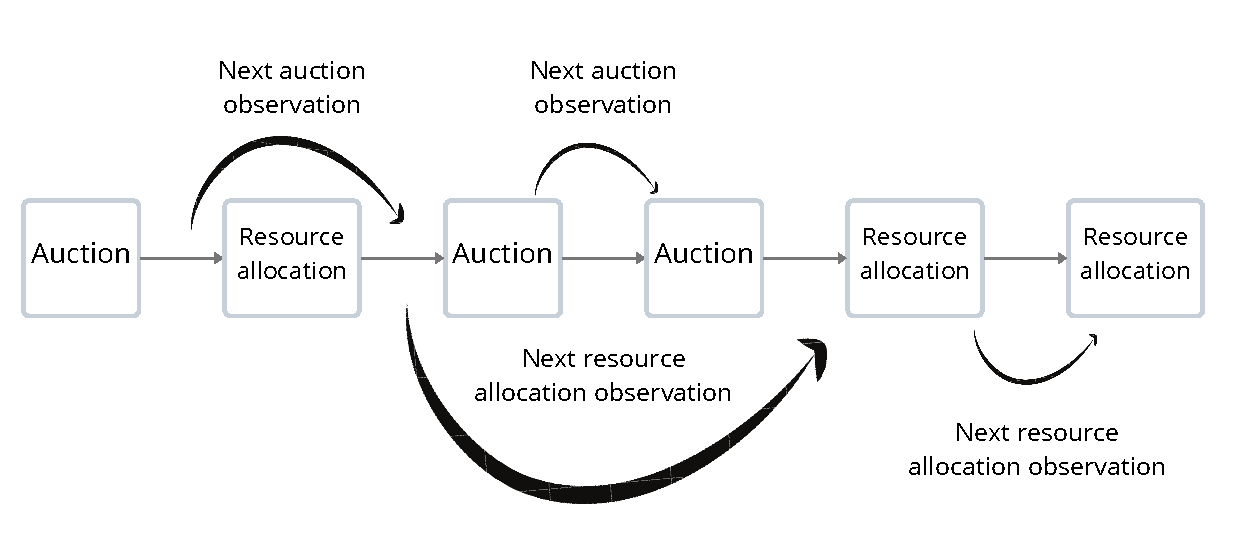
\includegraphics[width=14cm]{figures/env_server_agents_observations.pdf}
    \caption{Environment server agents observations}
    \label{fig:environment-observations}
\end{figure}

For the resource allocation agent, a trick is implemented such that the next observation for the agent is not the
actual next resource allocation observation as shown in the figure but a generated observation from the resulting
server state due to agent's actions. This is identical to the last case in the figure where no auction occurs between
resource allocation steps. Because of this, the resource allocation q value is able to approximate the reward for the
results of its actions directly and makes it appear to the agent that there is no auction steps with the observations
and next observations for training.
% Todo add number of tasks observations problems

For the auction agent, as the agent observations require an auction task to compare to and select an action (the task
bidding price), a trick like the one implemented for the resource allocation agent is not possible to implement.
Therefore during each server's last observation to recorded such that when the next auction occurs, this new task
observation can be used as the server's next observation. This is a suboptimal solution as the agent as the next task
been auctioned in completely random as well as between the current task observation and the next auction observation,
an unknown number of resource allocation steps could have been taken meaning that the resource demand by the other
currently allocated tasks has changed. A possible solution that has not been implement in this project is N step
prediction~\citep{multi-step-dqn} where the agent doesn't predict the q value of the next environment, but the q value
of the environment in N steps time. This is believed to help reduce the amount of randomness in the server's
observation to train on.

\section{Training agents}\label{sec:training-agents}
The first section of this chapter simulates edge cloud computing servers (section~\ref{sec:simulating-edge-cloud-computing-services})
while the second section implements auction and resource allocation agents that can interact with such environment
and use a range of algorithms to learn from. By combining both of these together allows agents to continually interact
with environments in order to learn over time their respective policies.

Neural networks, the bases of the reinforcement learning agents implemented, often require huge amounts of data and
high spec GPUs to run efficiently. Because of this, Iridis 5, University of Southampton supercomputer was utilised with
GTX1050 GPUs to train these agents for long periods of time and on mass. During training, for each episode a random
environment was generated from a list of possible settings in which the agents would be allocated to random servers. The
environment was run till the end, with the agent observation being added to their replay buffers after each actions
that were chosen epsilon greedily.

But after every 5 episodes, the agents would be evaluated using a set of environment that were pre-generated and
saved at the beginning of training. This allows the same environments over training in order to have a constant metric
in order to compare the agents over time. The actions taken are recorded to be used in evaluation
(chapter~\ref{ch:evaluation-of-the-implementation}) with the number of completed and failed tasks being stored about
the resource allocation agent and the winning prices being stored about the auction agents. Plus an action histograms
for each agents in order to view how agents bid and weightings are distributed.

% TODO Single resource allocation agent

\subsection{Agent training hyperparameters}\label{subsec:agent-training-hyperparameters}
% TODO

\begin{longtable}{|p{3.5cm}|p{3.5cm}|p{3.5cm}|p{3.5cm}|} \hline
    \textbf{Agent} & \textbf{Properties name} & \textbf{Value} & \textbf{Explanation} \\ \hline
        % TODO
        Task Pricing & limit\_parallel\_tasks & None & \\ \hline
        RL Agent & batch\_size &  32 & \\ \hline
        RL Agent & error\_loss\_fn & tf.losses.huber\_loss & \\ \hline
        RL Agent & initial\_training\_replay\_size & 5000 & \\ \hline
        RL Agent & training\_freq & 2 & \\ \hline
        RL Agent & discount\_factor & 0.9 & \\ \hline
        RL Agent & replay\_buffer\_length & 25000 & \\ \hline
        RL Agent & save\_frequency & 25000 & \\ \hline
        RL Agent & training\_loss\_log\_freq & 250 & \\ \hline \hline
        Task Pricing RL Agent & reward\_scaling & 1 & \\ \hline
        Task Pricing RL Agent & failed\_auction\_reward & -0.05 & \\ \hline
        Task Pricing RL Agent & failed\_multiplier & -1.5 & \\ \hline \hline
        Resource weighting RL Agent & other\_task\_discount: float = 0.4 & \\ \hline
        Resource weighting RL Agent & success\_reward & 1 & \\ \hline
        Resource weighting RL Agent & failed\_reward & -1.5 & \\ \hline \hline
        Dqn Agent & optimiser & tf.keras.optimizers.Adam() & \\ \hline
        Dqn Agent & target\_update\_tau & 1.0 & \\ \hline
        Dqn Agent & target\_update\_frequency & 2500 & \\ \hline
        Dqn Agent & initial\_epsilon & 1 & \\ \hline
        Dqn Agent & final\_epsilon & 0.1 & \\ \hline
        Dqn Agent & epsilon\_steps & 10000 & \\ \hline
        Dqn Agent & epsilon\_update\_frequency & 100 & \\ \hline \hline
        Dueling Dqn Agent & double\_loss & True & \\ \hline \hline
        Categorical Dqn Agent & max\_value & -20.0 & \\ \hline
        Categorical Dqn Agent & min\_value & 25.0 & \\ \hline
        Categorical Dqn Agent & num\_atoms & 21 & \\ \hline \hline
        Ddpg Agent & actor\_optimiser & tf.keras.optimizers.RMSprop(lr=0.0001) & \\ \hline
        Ddpg Agent & critic\_optimiser & tf.keras.optimizers.RMSprop(lr=0.0005) & \\ \hline
        Ddpg Agent & initial\_epsilon\_std & 0.8 & \\ \hline
        Ddpg Agent & final\_epsilon\_std & 0.05 & \\ \hline
        Ddpg Agent & epsilon\_steps & 20000 & \\ \hline
        Ddpg Agent & epsilon\_update\_frequency & 100 & \\ \hline
        Ddpg Agent & target\_update\_tau & 1.0 & \\ \hline
        Ddpg Agent & actor\_target\_update\_frequency & 3000 & \\ \hline
        Ddpg Agent & critic\_target\_update\_frequency & 1500 & \\ \hline
        Ddpg Agent & upper\_action\_bound & 30.0 & \\ \hline \hline
        Task pricing Ddpg Agent & min\_value & -100.0 & \\ \hline
        Task pricing Ddpg Agent & max\_value & 100.0 & \\ \hline \hline
        Resource allocation Ddpg Agent & min\_value & -20 & \\ \hline
        Resource allocation Ddpg Agent & max\_value & 15 & \\ \hline \hline
        TD3 Agent & twin\_critic\_optimiser & tf.keras.optimizers.Adam() & \\ \hline
        TD3 Agent & actor\_update\_frequency & 3 & \\ \hline
    \caption{Agent hyperparameters}
    \label{tab:agent_hyperparameters}
\end{longtable}


